\documentclass[12pt]{article}
\usepackage[utf8]{inputenc}
\usepackage[margin=1in]{geometry}
\usepackage{amsmath}\usepackage{amssymb}\usepackage{multicol}\usepackage{enumitem}
\usepackage{pgfplots}\pgfplotsset{compat=1.17}
\setlength{\parindent}{0pt}
\begin{document}

\fbox{\parbox{0.97\linewidth}{\small\textbf{Final answers} (record here --- graded on the answer; show your work):\\[6pt]1.~\underline{\hspace{1.5cm}}\quad 2.~\underline{\hspace{1.5cm}}\quad 3.~\underline{\hspace{1.5cm}}\quad 4.~\underline{\hspace{1.5cm}}\quad 5.~\underline{\hspace{1.5cm}}\quad 6.~\underline{\hspace{1.5cm}}\quad 7.~\underline{\hspace{1.5cm}}\quad 8.~\underline{\hspace{1.5cm}}\quad 9.~\underline{\hspace{1.5cm}}\quad 10.~\underline{\hspace{1.5cm}}}}
\vspace{0.35cm}

\begin{center}{\Large \textbf{Warm-Up: Max or Min?}}\end{center}\vspace{0.2cm}
% Warm-Up: Max or Min?
\textbf{Example (Warm-Up: Max or Min?):}

For $y=4(x-2)^2+7$, since $a=4>0$, the function has a minimum value of $7$.

\vspace{0.2cm}\hrule\vspace{0.35cm}
\textbf{Directions: State whether each function has a maximum or minimum, and give that value.}

\begin{multicols}{2}
\begin{enumerate}[label=\textbf{\arabic*.}, start=1, itemsep=1.3cm]
  \item $\displaystyle y=-2(x+1)^2+10$
  \item $\displaystyle y=5(x-3)^2-6$
  \item $\displaystyle y=-(x-4)^2+1$
  \item $\displaystyle y=\frac{1}{2}(x+2)^2-8$
\end{enumerate}
\end{multicols}
\vspace{0.25cm}\hrule\vspace{0.35cm}

\begin{center}{\Large \textbf{Find the Vertex from Standard Form}}\end{center}\vspace{0.2cm}
% Find the Vertex from Standard Form
\textbf{Example (Find the Vertex from Standard Form):}

For $y=-3x^2+12x+2$, find $x=-\dfrac{b}{2a}=-\dfrac{12}{2(-3)}=2$, then $y=-3(2)^2+12(2)+2=14$. Maximum value is 14.

\vspace{0.2cm}\hrule\vspace{0.35cm}
\textbf{Directions: Find the x-coordinate of the vertex, then the max/min value for each function.}

\begin{multicols}{2}
\begin{enumerate}[label=\textbf{\arabic*.}, start=5, itemsep=2cm]
  \item $\displaystyle y=-x^2+6x-3$
  \item $\displaystyle y=2x^2-8x+5$
  \item $\displaystyle y=-4x^2+16x+1$
\end{enumerate}
\end{multicols}
\vspace{0.25cm}\hrule\vspace{0.35cm}

\begin{center}{\Large \textbf{Real-World Applications}}\end{center}\vspace{0.2cm}
% Real-World Applications
\textbf{Example (Real-World Applications):}

A vendor's profit is $P(x)=-x^2+30x-50$, where $x$ is the price in dollars. The vertex occurs at $x=-\dfrac{30}{-2}=15$, giving $P(15)=175$. The maximum profit is $175 dollars at a price of $15.

\begin{center}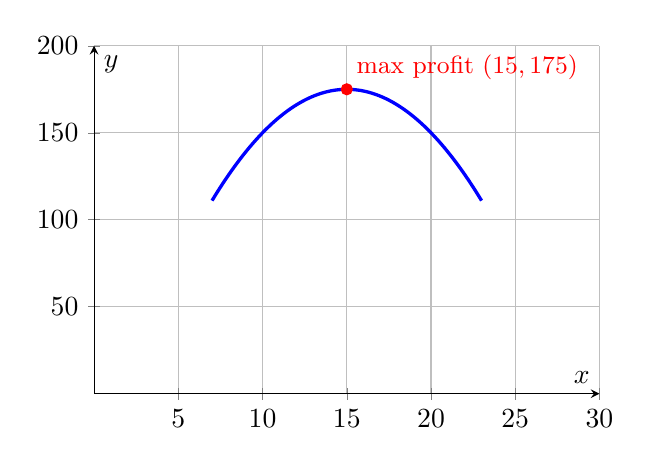
\begin{tikzpicture}
\begin{axis}[axis lines=middle,xlabel=$x$,ylabel=$y$,xmin=0,xmax=30,ymin=0,ymax=200,width=8cm,height=6cm,grid=both,samples=80]
\addplot[very thick,blue,domain=7:23]{-1*(x-15)^2+175};
\addplot[only marks,mark=*,red] coordinates {(15,175)};
\node[above right,red,font=\small] at (axis cs:15,175) {max profit $(15,175)$};
\end{axis}\end{tikzpicture}\end{center}
{\small\centering Profit model $P(x)=-x^2+30x-50$ reaching a maximum of \textbackslash\{\}$175 at $x=15\$.\par}
\vspace{0.2cm}\hrule\vspace{0.35cm}
\textbf{Directions: Set up the vertex for each model, find the max/min value, and interpret the result in a full sentence with units.}

\begin{multicols}{2}
\begin{enumerate}[label=\textbf{\arabic*.}, start=8, itemsep=3cm]
  \item A rocket's height is $h(t)=-16t^2+96t+10$ (feet, $t$ in seconds). Find the maximum height and when it occurs.
  \item A rectangular pen against a barn uses 60 ft of fencing on 3 sides: $A(x)=-2x^2+60x$. Find the maximum area and the width that produces it.
\end{enumerate}
\end{multicols}

\vspace{0.2cm}\hrule\vspace{0.3cm}
\textbf{Challenge} (same sheet):\\[4pt]
\begin{enumerate}[label=\textbf{\arabic*.}, start=10, itemsep=2.2cm]
  \item A company's cost to produce $x$ items is $C(x)=2x^2-40x+300$. Find the minimum cost and the number of items that produce it.
\end{enumerate}

\newpage

\begin{center}{\Large \textbf{Answer Key --- fully worked}}\end{center}
\vspace{0.25cm}
\textbf{Procedure:} Determine whether the function opens up (minimum) or down (maximum) from the sign of $a$.; Find the x-coordinate of the vertex using $x=h$ (vertex form) or $x=-\dfrac{b}{2a}$ (standard form).; Substitute that x-value back into the function to find the max/min value, $k$.; Interpret the result in the context of the problem, including correct units.; State your final answer as a full sentence: the maximum/minimum [quantity] is [value], occurring at [x-value]..\\[8pt]
\begin{enumerate}[label=\textbf{\arabic*.},itemsep=7pt]
  \item Maximum value of $10$ (since $a=-2<0$).
  \item Minimum value of $-6$ (since $a=5>0$).
  \item Maximum value of $1$ (since $a=-1<0$).
  \item Minimum value of $-8$ (since $a=\frac{1}{2}>0$).
  \item $x=-\frac{6}{-2}=3$; $y=-9+18-3=6$. Maximum value is $6$.
  \item $x=-\frac{-8}{4}=2$; $y=8-16+5=-3$. Minimum value is $-3$.
  \item $x=-\frac{16}{-8}=2$; $y=-16+32+1=17$. Maximum value is $17$.
  \item $t=-\frac{96}{-32}=3$; $h(3)=-144+288+10=154$. The maximum height is 154 feet, occurring at 3 seconds.
  \item $x=-\frac{60}{-4}=15$; $A(15)=-450+900=450$. The maximum area is 450 square feet, occurring when the width is 15 feet.
  \item $C(x)=2x^2-40x+300$ has $a=2>0$, so it opens up and has a minimum. Vertex x-coordinate: $x=-\frac{-40}{2(2)}=\frac{40}{4}=10$. Minimum cost: $C(10)=2(10)^2-40(10)+300=200-400+300=100$. The minimum cost is \$100, achieved when 10 items are produced.
\end{enumerate}

\end{document}